\documentclass[aspectratio=169,11pt]{beamer}

\usetheme{default}
\usecolortheme{seahorse}
\setbeamertemplate{navigation symbols}{}
\setbeamertemplate{footline}[frame number]

\usepackage{graphicx}
\usepackage{booktabs}
\usepackage{amsmath}

\graphicspath{{../plots/}{../prototype/mini_p1d/docs/figures/}}

\title{Analytic Lyman-alpha \(P_{1\mathrm{D}}\)}
\subtitle{Pipeline, FGPA, and what comes next}
\author{Helena}
\date{Tuesday 13 October 2026}

\begin{document}

\begin{frame}
  \titlepage
\end{frame}

\begin{frame}{The task}
  \begin{itemize}
    \item Input: \(n_s\), \(A_s\), and \(P_\mathrm{CDM}(k)\).
    \item Output: \(P_{1\mathrm{D}}(k,z)\), with \(k\) in s/km and power in km/s.
    \item \(P_\mathrm{CDM}\) can be Eisenstein--Hu, a table, or an \(\alpha\beta\gamma\delta\) bend.
    \item \(P_x\), the covariance, and the Fisher matrix are the next stage.
  \end{itemize}
  \vspace{0.6em}
  The function to call is \texttt{p1d\_skm}.\\
  Repository: \texttt{garciaeh77/fisher-forecasts-future-spectroscopic-survey}
\end{frame}

\begin{frame}{What I built}
  \begin{enumerate}
    \item Build \(P_\mathrm{CDM}(k,z)\).
    \item Turn that spectrum into flux with the FGPA.
    \item Integrate along the line of sight and convert to forest units.
  \end{enumerate}
  \vspace{0.8em}
  Two flux models share the same \(P_\mathrm{CDM}\).
  \begin{itemize}
    \item Kaiser formula: the fast \(P_{1\mathrm{D}}\) for a later Fisher forecast.
    \item Optical-depth skewers: a check of that formula.
  \end{itemize}
\end{frame}

\begin{frame}{The four stages}
  \centering
  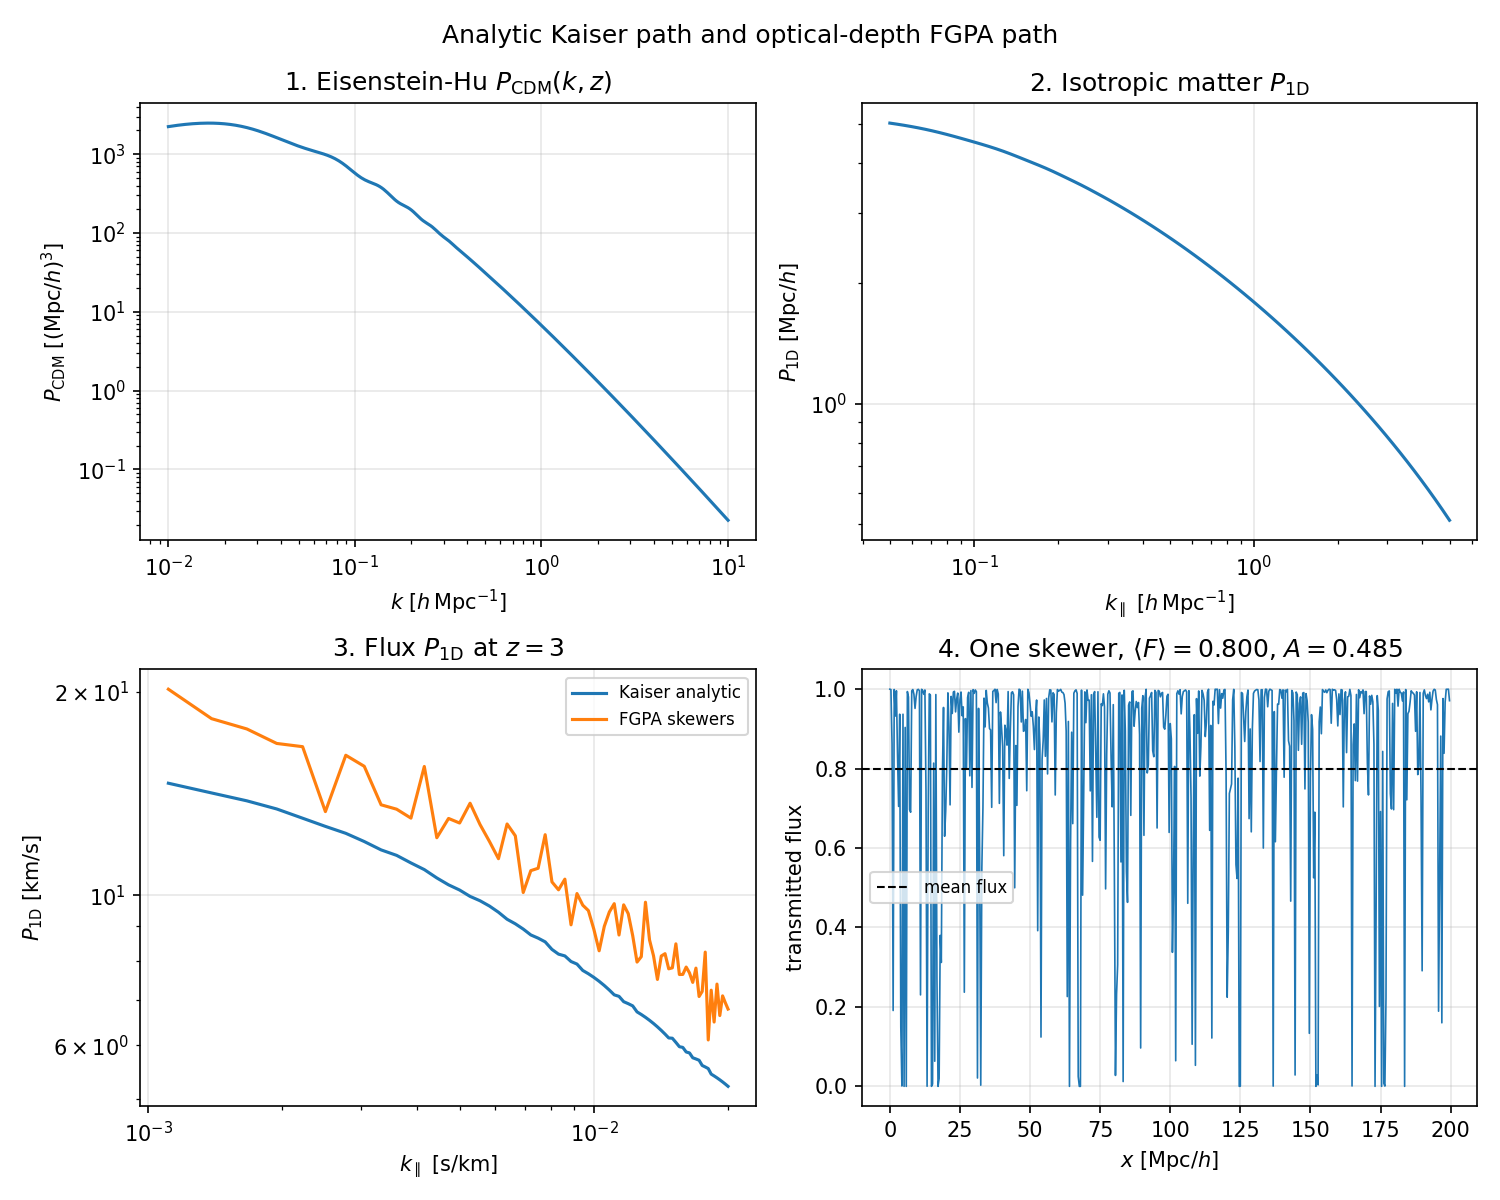
\includegraphics[width=0.92\textwidth,height=0.78\textheight,keepaspectratio]{07_pipeline_stages.png}
\end{frame}

\begin{frame}{Stage 1: Eisenstein--Hu \(P_\mathrm{CDM}\)}
  \[
    P_\mathrm{CDM}(k,z)
    = A_s\left(\frac{k}{k_\mathrm{pivot}}\right)^{n_s-1} T_\mathrm{EH}^2(k)\,D(z)^2
  \]
  \begin{itemize}
    \item \(T(k)\) is Eisenstein \& Hu (1998), with baryon wiggles. \(T(k\to 0)=1\).
    \item Pivot \(k=0.05\,\mathrm{Mpc}^{-1}\).
    \item Against CAMB, the median ratio is about \(1.01\) from \(10^{-3}\) to \(10\,h\,\mathrm{Mpc}^{-1}\).
  \end{itemize}
\end{frame}

\begin{frame}{\(n_s\) tilts \(P_\mathrm{CDM}\). \(A_s\) rescales it.}
  \centering
  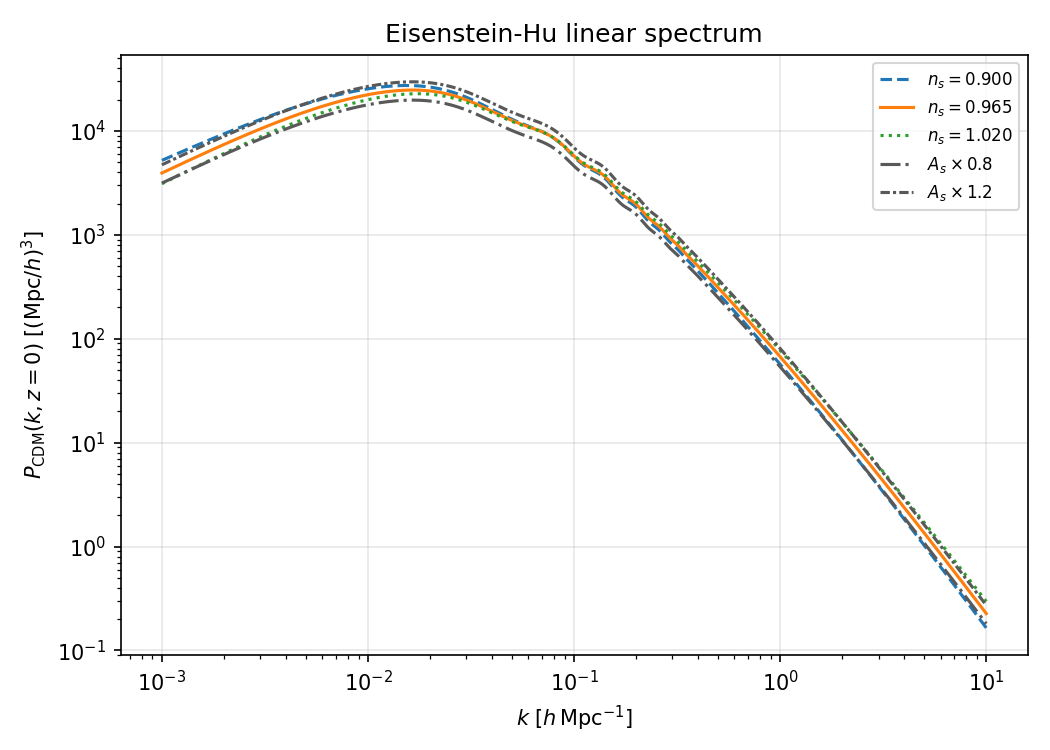
\includegraphics[width=0.78\textwidth,height=0.78\textheight,keepaspectratio]{01_pcdm_ns_As.png}
\end{frame}

\begin{frame}{The same changes, after the projection to \(P_{1\mathrm{D}}\)}
  \centering
  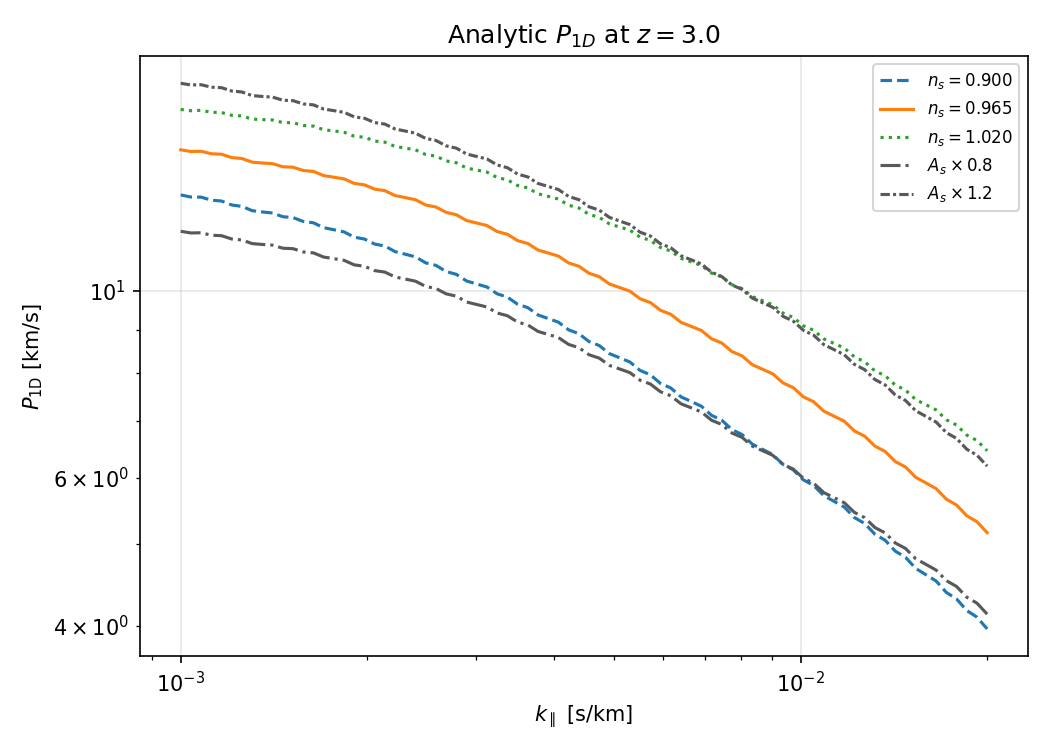
\includegraphics[width=0.78\textwidth,height=0.78\textheight,keepaspectratio]{02_p1d_ns_As.png}
\end{frame}

\begin{frame}{Where the FGPA enters: the Kaiser path}
  The full model is \(\tau = A(\rho/\bar\rho)^\beta\) and \(F=e^{-\tau}\),
  with \(\beta = 2 - 0.7(\gamma-1)\).
  \vspace{0.5em}
  For small fluctuations this becomes
  \[
    P_F(k,\mu,z) = b_F^2\,(1+\beta_F\mu^2)^2\,P_\mathrm{CDM}(k,z),
  \]
  with \(b_F=-0.14\), \(\beta_F=1.4\), and \(\mu=k_\parallel/k\).
  \vspace{0.4em}
  \(b_F\) is negative because a denser patch transmits less flux.
  Both numbers are fixed. This path does not build a skewer.
\end{frame}

\begin{frame}{Line-of-sight integral}
  \[
    P_{1\mathrm{D}}(k_\parallel)
    = \int_{k_\parallel}^{k_\mathrm{max}}
      \frac{k\,\mathrm{d}k}{2\pi}\,
      P_F\!\left(k,\mu=\frac{k_\parallel}{k}\right)
  \]
  \begin{itemize}
    \item \(k_\mathrm{max}=30\,h\,\mathrm{Mpc}^{-1}\).
    \item Then multiply by \(H(z)/((1+z)h)\) to get km/s.
    \item Input \(k_\parallel\) is in s/km.
  \end{itemize}
\end{frame}

\begin{frame}{Check: \(A_s\) is a pure amplitude. \(n_s\) tilts.}
  \centering
  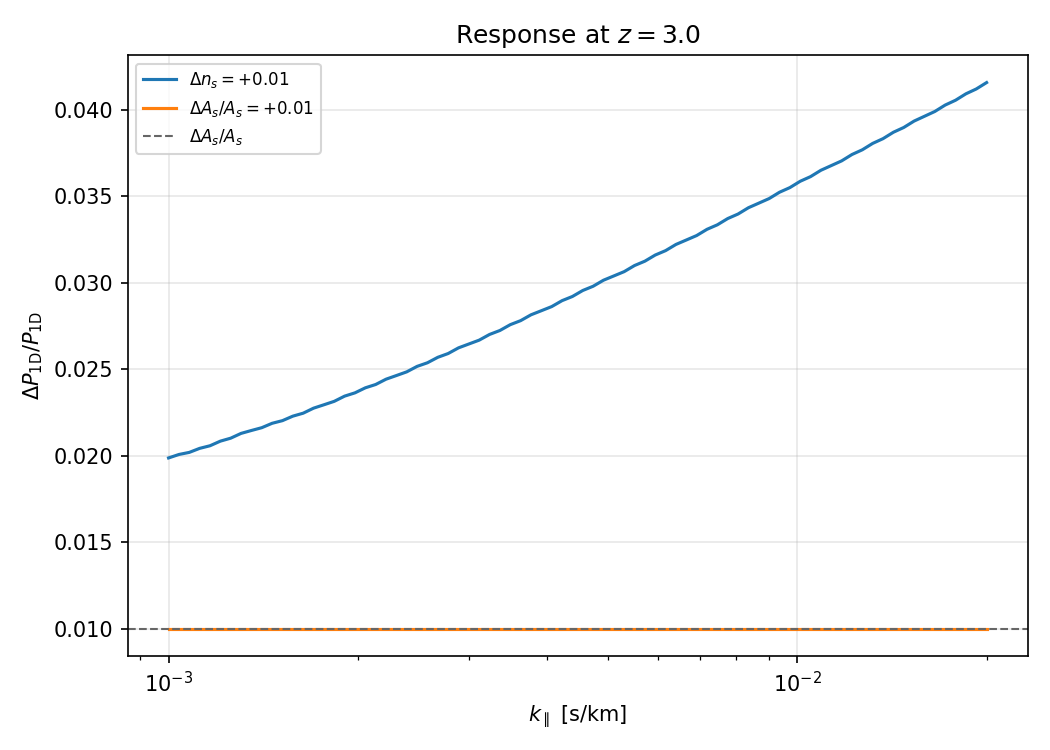
\includegraphics[width=0.78\textwidth,height=0.78\textheight,keepaspectratio]{03_p1d_fractional.png}
\end{frame}

\begin{frame}{Redshift at fixed cosmology}
  \centering
  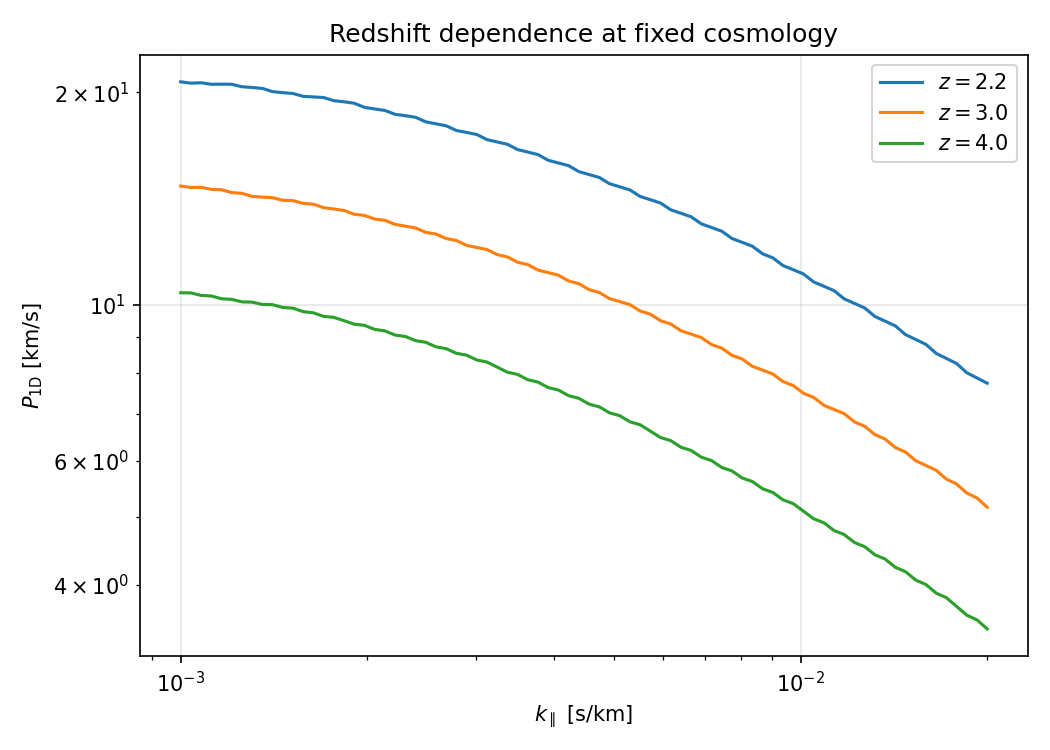
\includegraphics[width=0.78\textwidth,height=0.78\textheight,keepaspectratio]{04_p1d_redshifts.png}
\end{frame}

\begin{frame}{\(P_\mathrm{CDM}\) can also be read from a file}
  Rescaling of a stored table:
  \[
    P(k) = P_\mathrm{fid}(k)\,
    \frac{A_s}{A_{s,\mathrm{fid}}}
    \left(\frac{k}{k_p}\right)^{n_s-n_{s,\mathrm{fid}}}
    \left(\frac{D}{D_\mathrm{fid}}\right)^2
  \]
  The code refuses \(k\) outside the table.
\end{frame}

\begin{frame}{The table matches a direct Eisenstein--Hu call}
  \centering
  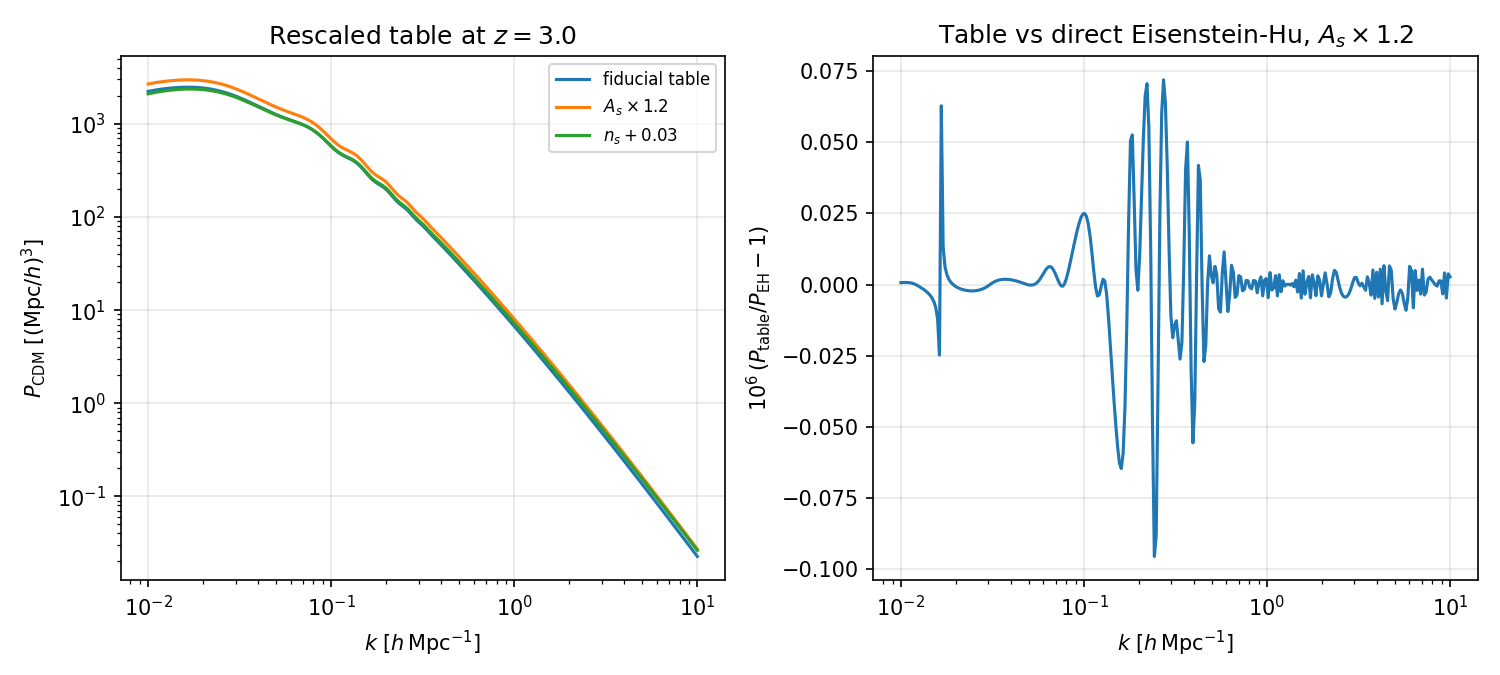
\includegraphics[width=0.92\textwidth,height=0.78\textheight,keepaspectratio]{06_table_rescaling.png}
\end{frame}

\begin{frame}{The \(\alpha\beta\gamma\delta\) bend}
  With \(L=\ln(k/k_p)\) and \(k_p=1\,h\,\mathrm{Mpc}^{-1}\),
  \[
    P(k)=P_\mathrm{EH}(k)\,
    \exp(\alpha L+\beta L^2+\gamma L^3+\delta L^4).
  \]
  At the pivot the exponential is 1.
  All four coefficients set to zero returns Eisenstein--Hu.
\end{frame}

\begin{frame}{One coefficient at a time}
  \centering
  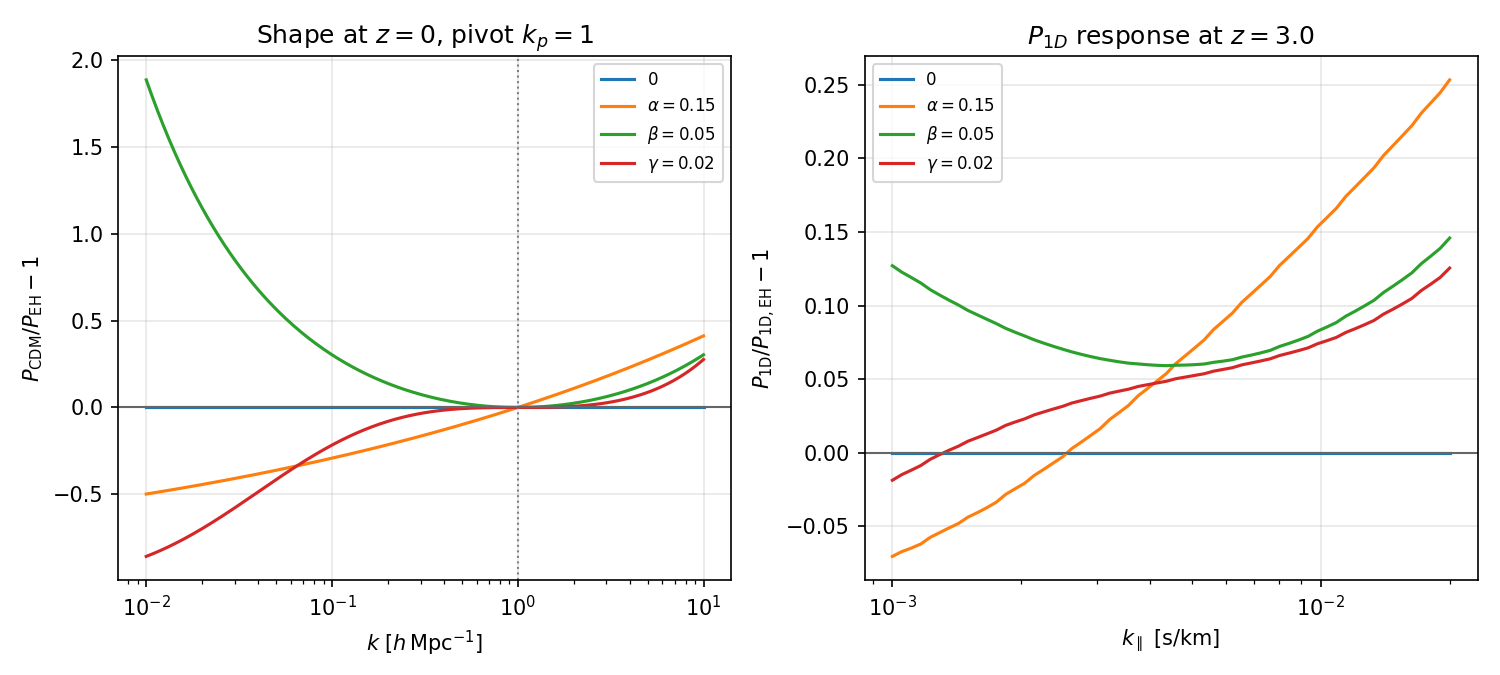
\includegraphics[width=0.92\textwidth,height=0.78\textheight,keepaspectratio]{05_abgd_shape.png}
\end{frame}

\begin{frame}{The second FGPA: optical depth on skewers}
  \begin{enumerate}
    \item Draw Gaussian skewers from the matter \(P_{1\mathrm{D}}\).
    \item Map them to a lognormal density \(\Delta\).
    \item Set \(\tau = A\Delta^\beta\), with \(\beta=2-0.7(\gamma-1)\).
    \item Solve for \(A\) so the mean flux is \(0.80\).
  \end{enumerate}
  \vspace{0.4em}
  At \(\gamma=1.5\): \(\beta=1.65\) and \(A=0.485\).
  Pressure smoothing and thermal broadening are in the code and switched off.
\end{frame}

\begin{frame}{Shapes agree. Absolute amplitudes do not.}
  \centering
  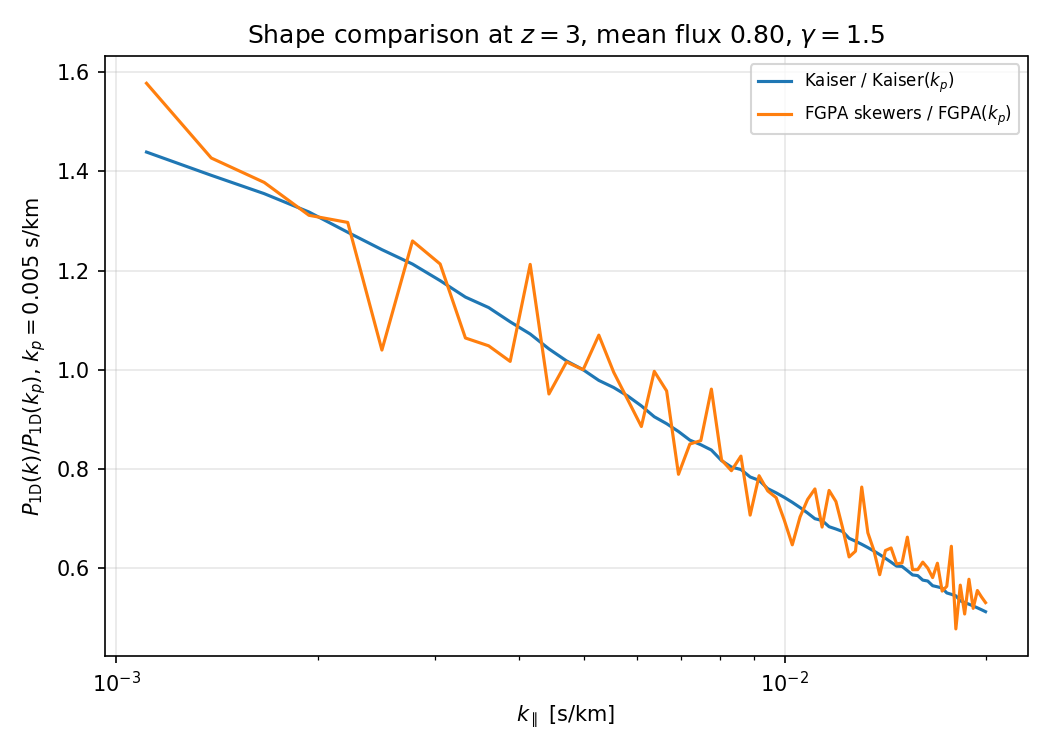
\includegraphics[width=0.78\textwidth,height=0.78\textheight,keepaspectratio]{08_kaiser_vs_fgpa_shape.png}
\end{frame}

\begin{frame}{What is not in the repository yet}
  \begin{itemize}
    \item \(P_x\), the forest--tracer cross-power.
    \item The covariance.
    \item The Fisher matrix.
  \end{itemize}
  \vspace{0.6em}
  The Kaiser \(P_{1\mathrm{D}}\) is the signal those three pieces would use.
  The skewer path is the check, not the derivative.
\end{frame}

\begin{frame}{Questions before the next stage}
  \begin{enumerate}
    \item Is \(P_x\) the cross with quasars, galaxies, or both, and is it \(P_x(k,\mu,z)\)?
    \item Is the first covariance 1D \(P_{1\mathrm{D}}\), or 3D \(C=2P_T^2/N_k\)?
    \item Which knobs enter first: area, densities, resolution, signal-to-noise?
    \item Are the free Fisher parameters only \(n_s\) and \(A_s\), with biases fixed?
  \end{enumerate}
\end{frame}

\appendix
\begin{frame}{Backup: the other prototype}
  The original package is stored unchanged in \texttt{prototype/mini\_p1d/}.
  \vspace{0.6em}
  Its two figures are
  \begin{itemize}
    \item \texttt{docs/figures/matter\_power\_comparison.png}
    \item \texttt{docs/figures/flux\_p1d\_comparison.png}
  \end{itemize}
  They use that code's demonstration spectrum, not Eisenstein--Hu.
  The forecast pipeline is the combined version in \texttt{p1d/}.
\end{frame}

\end{document}
